\subsection{M.PC.AC - Actual Cost}

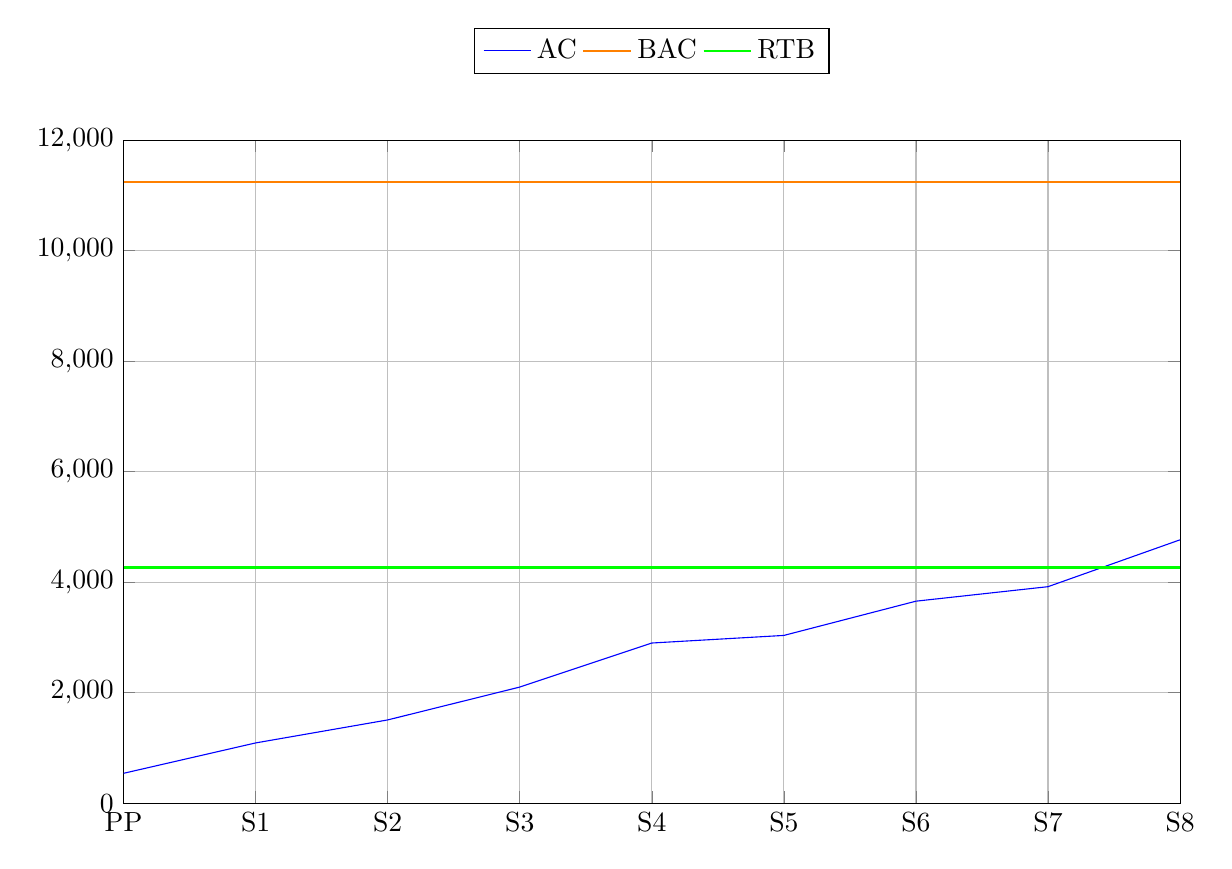
\begin{tikzpicture}
    \begin{axis}[
        width=15cm, height=10cm,
        ymin=0, ymax=12000,
        xmin=0, xmax=8,
        xtick={0, 1, 2, 3, 4, 5, 6, 7, 8},
        xticklabels={ PP, S1, S2, S3, S4, S5, S6, S7, S8},
        xlabel={},
        ylabel={},
        grid=major,
        scaled ticks=false,
        legend style={at={(0.5,1.1)}, anchor=south, legend columns=-1},
    ]
    \addplot[color=blue] coordinates {(0, 540) (1, 1090) (2, 1506.25) (3, 2101.25) (4, 2898.75) (5, 3036.25) (6, 3656.25) (7, 3918.75) (8, 4767.5)};
    \addlegendentry{AC}
    \addplot[orange, thick] coordinates {(0, 11250) (8, 11250)};
    \addlegendentry{BAC}
    \addplot[green, thick] coordinates {(0, 4265) (8, 4265)};
    \addlegendentry{RTB}
    \end{axis}
\end{tikzpicture}
\subsubsection{RTB}
Il grafico mostra l'incremento progressivo dei costi totali sostenuti a ogni \glossario{sprint}, 
includendo sia i costi per le attività completate sia quelli per le attività ancora in corso.